% Slides for 2024-07-16
% To create a slide, use the following:
% \begin{frame}{TITLE}
%     BODY
% \end{frame}


% To create a slide with a bullet list, use the following:

\begin{frame}{Results: Labelling Party - ROC Curve}
    \centering
    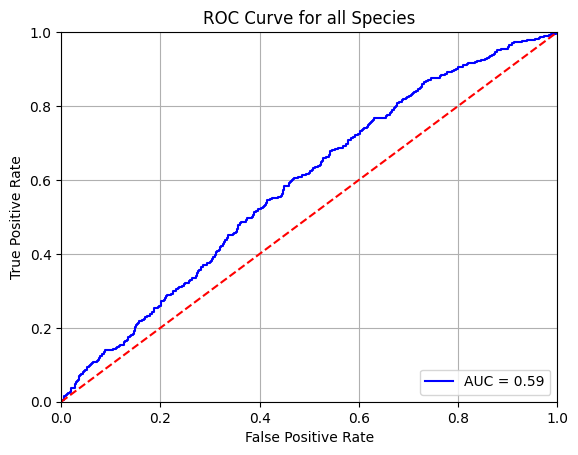
\includegraphics[height=0.9\textheight,width=0.9\textwidth,keepaspectratio]{images/ROC_Curve_original_grid.png}   
\end{frame}

\begin{frame}{Results: Labelling Party - AUC vs Time}
    \centering
    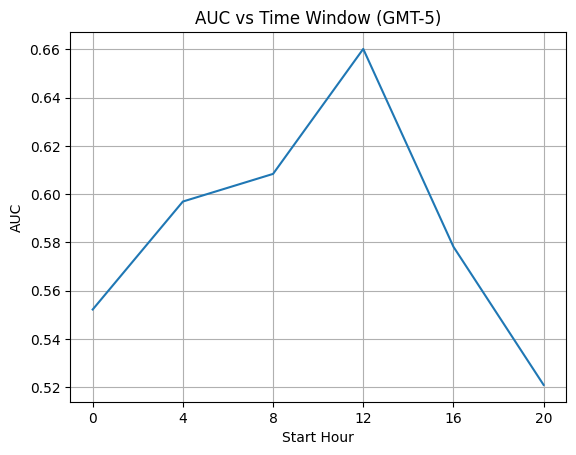
\includegraphics[height=0.9\textheight,width=0.9\textwidth,keepaspectratio]{images/AUC.png}   
\end{frame}

\begin{frame}{Results: Same model with strong Data Augmentation}
    \centering
    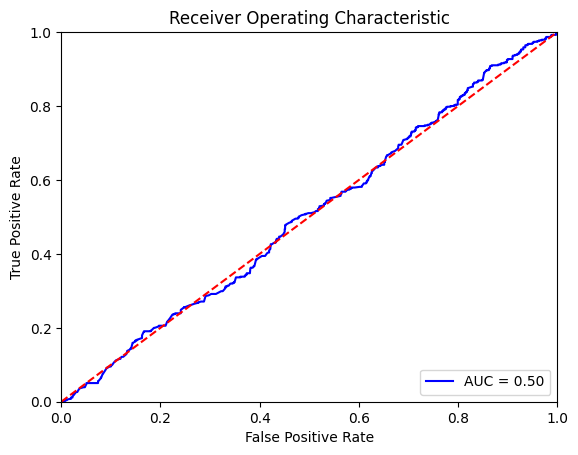
\includegraphics[height=0.9\textheight,width=0.9\textwidth,keepaspectratio]{images/ROC_Curve_DA.png}   
\end{frame}

\begin{frame}{Results: Same model with strong Data Augmentation}
    \centering
    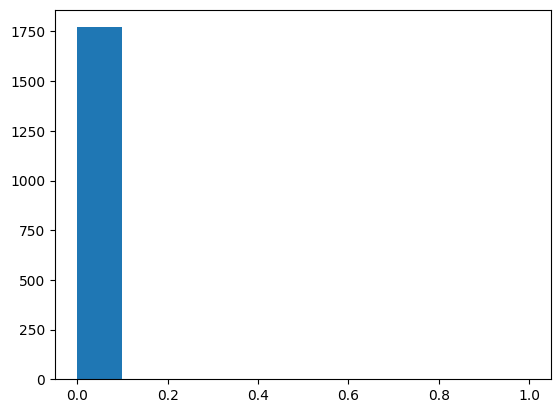
\includegraphics[height=0.9\textheight,width=0.9\textwidth,keepaspectratio]{images/distribution_DA.png}   
\end{frame}



\begin{frame}{Data Analysis}
    \begin{itemize}
        \item Class Correlation Matrix
        \item ITEM 2
    \end{itemize}    
\end{frame}

\begin{frame}{Class Correlation Matrix}
    \begin{itemize}
        \item Compute R for every pair of classes across all instances
        \item Goal: Find correlations (confusions)
    \end{itemize}    
\end{frame}

% picture of matrix, without filtering the zeros
\begin{frame}{Results: Class Correlation Matrix}
    \centering
    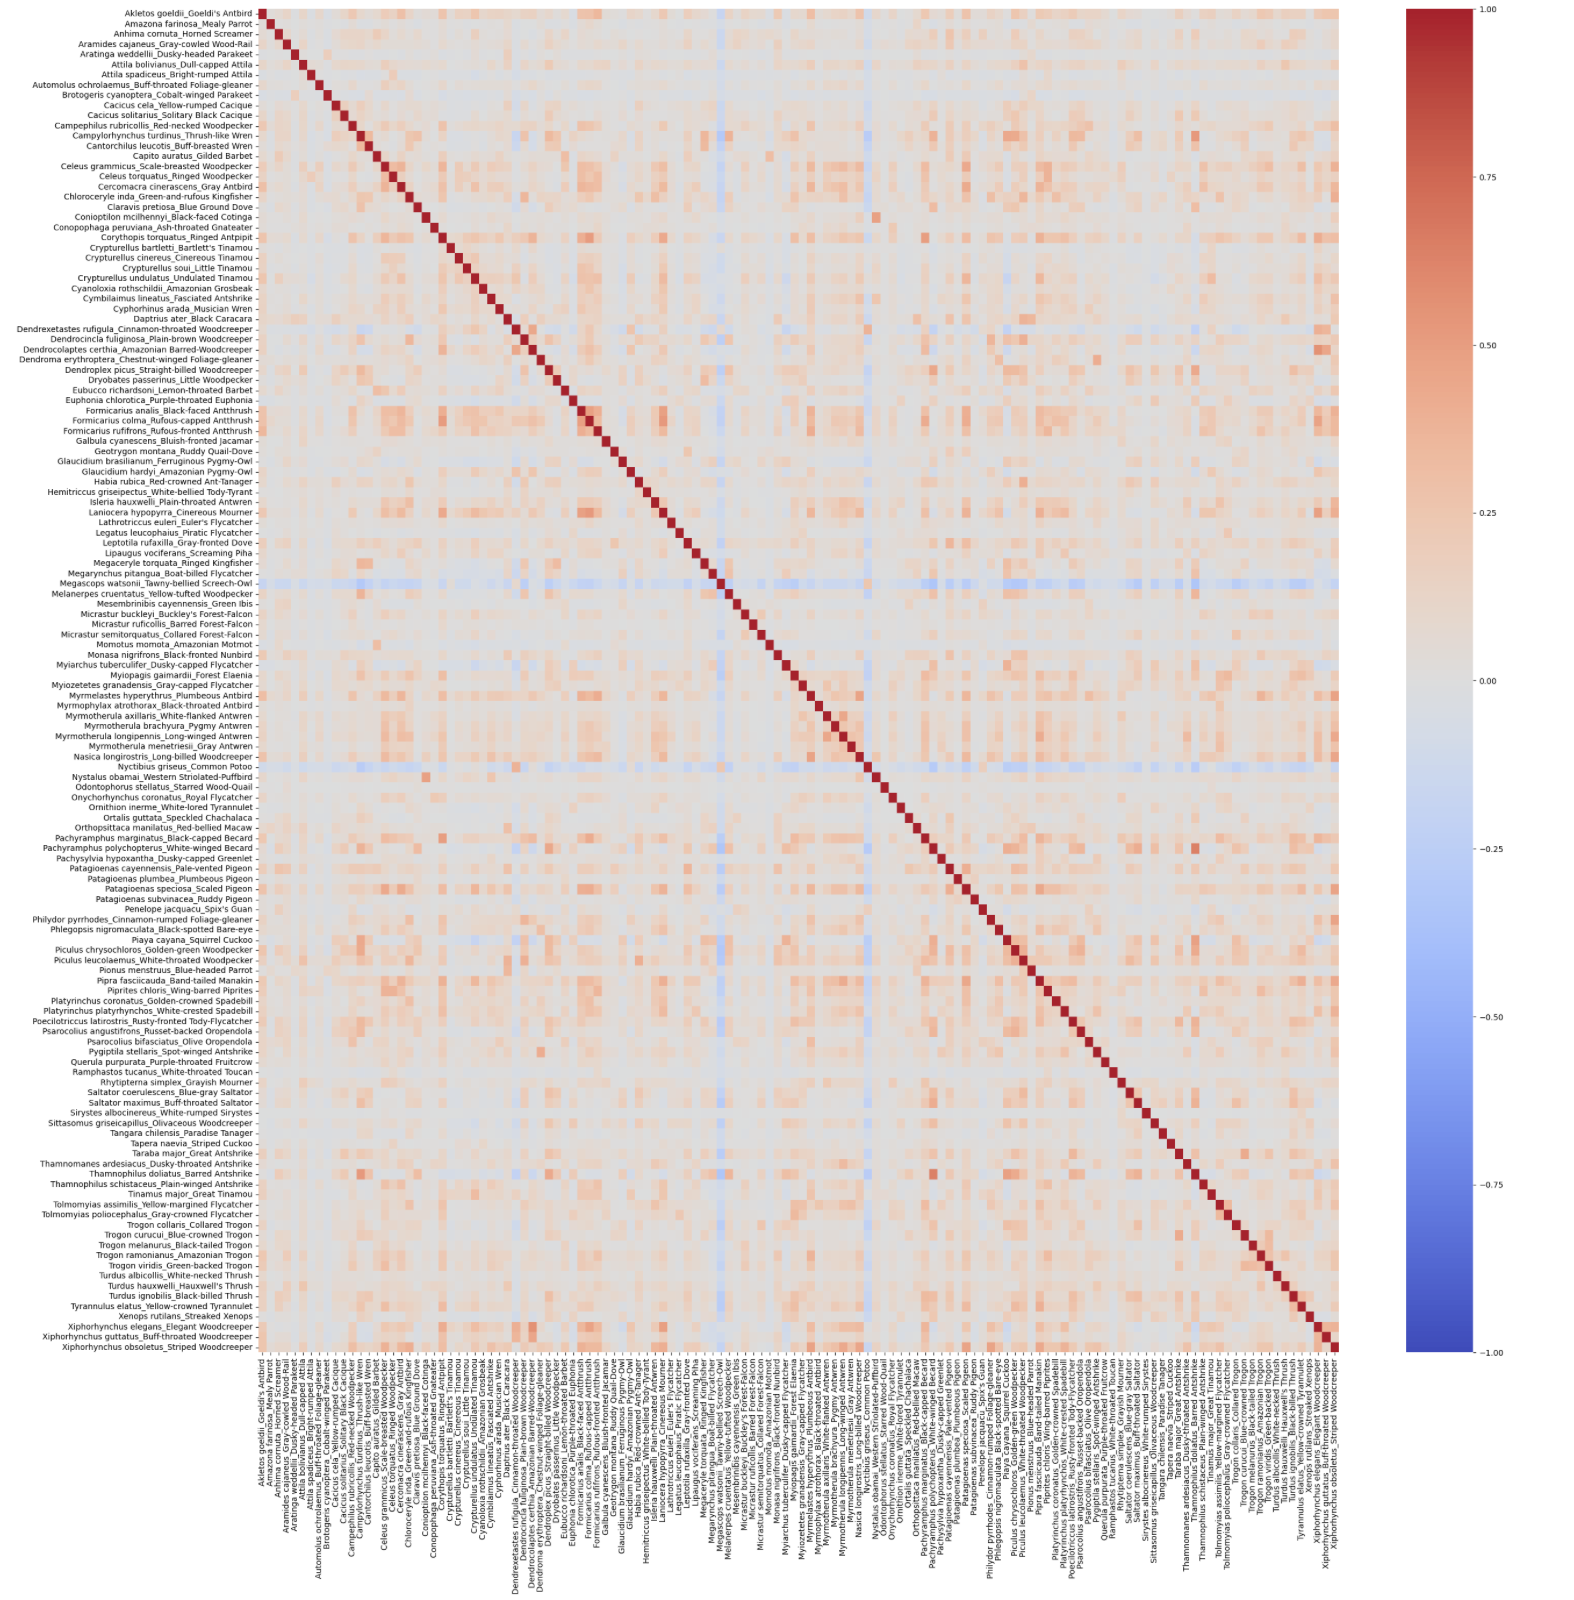
\includegraphics[height=0.9\textheight,width=0.9\textwidth,keepaspectratio]{images/no_filter.png}   
\end{frame}

% picture of matrix, with filtering the zeros
\begin{frame}{TITLE}
    \begin{columns}
        \begin{column}{0.5\textwidth}
            \centering
            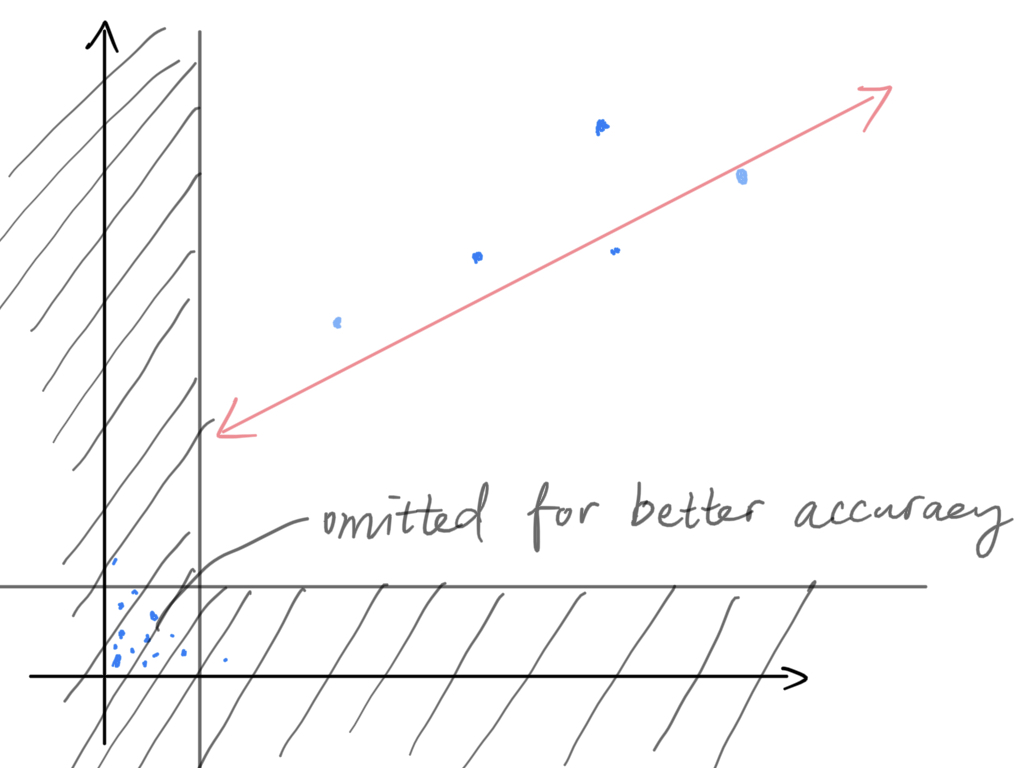
\includegraphics[height=0.9\textheight,width=0.9\textwidth,keepaspectratio]{images/conf_filter_explanation.jpeg}   
        \end{column}
        \begin{column}{0.5\textwidth}
            \centering
            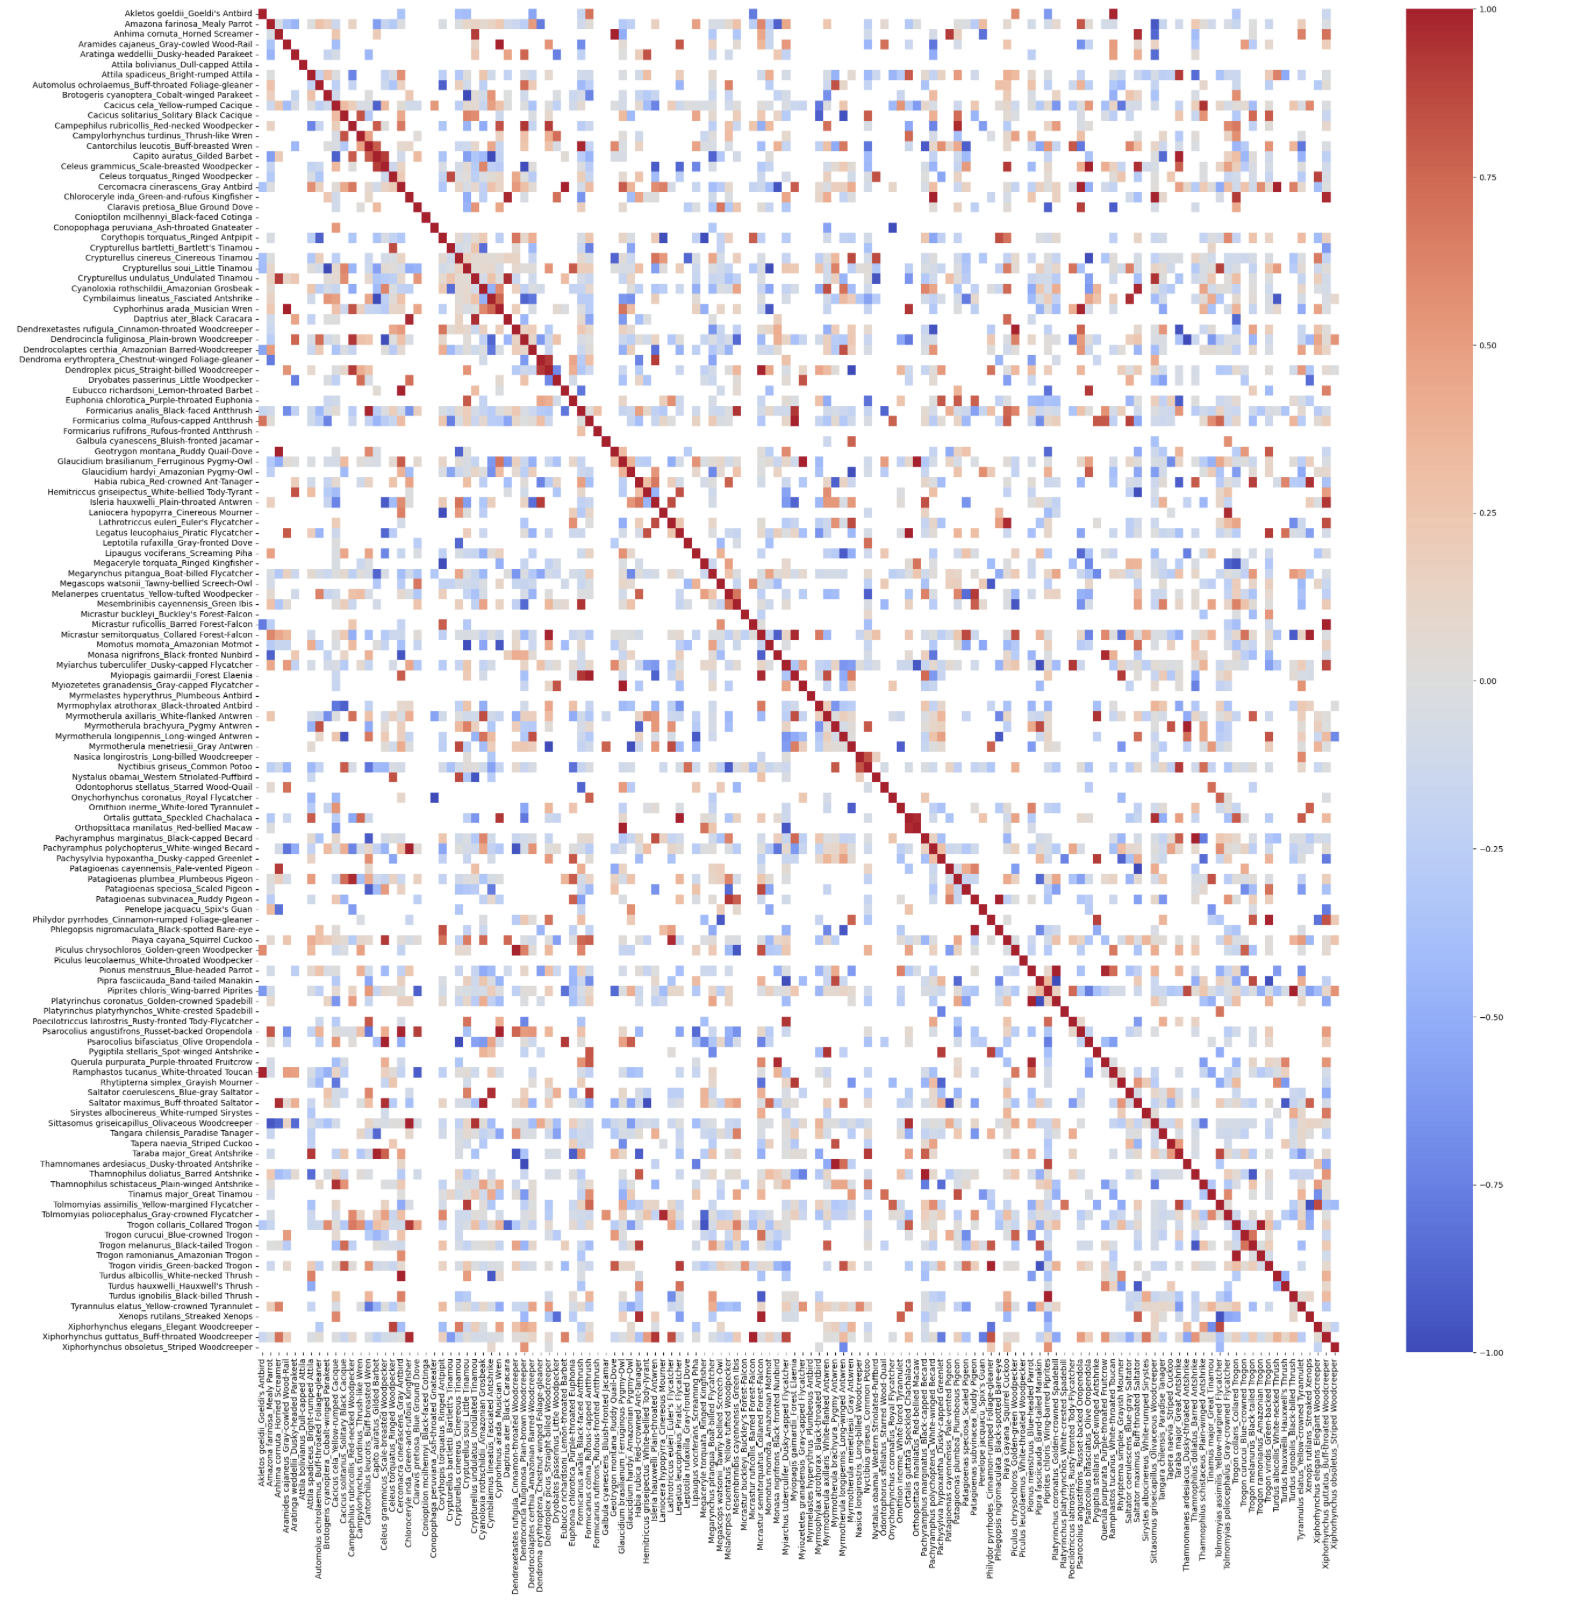
\includegraphics[height=0.9\textheight,width=0.9\textwidth,keepaspectratio]{images/confidence_filter.png} 
        \end{column}
    \end{columns}
\end{frame}


% picture of matrix, with filtering the number of datapoints
\begin{frame}{Results: Class Correlation Matrix}
    \centering
    White = Not enough datapoints
    \\
    \centering
    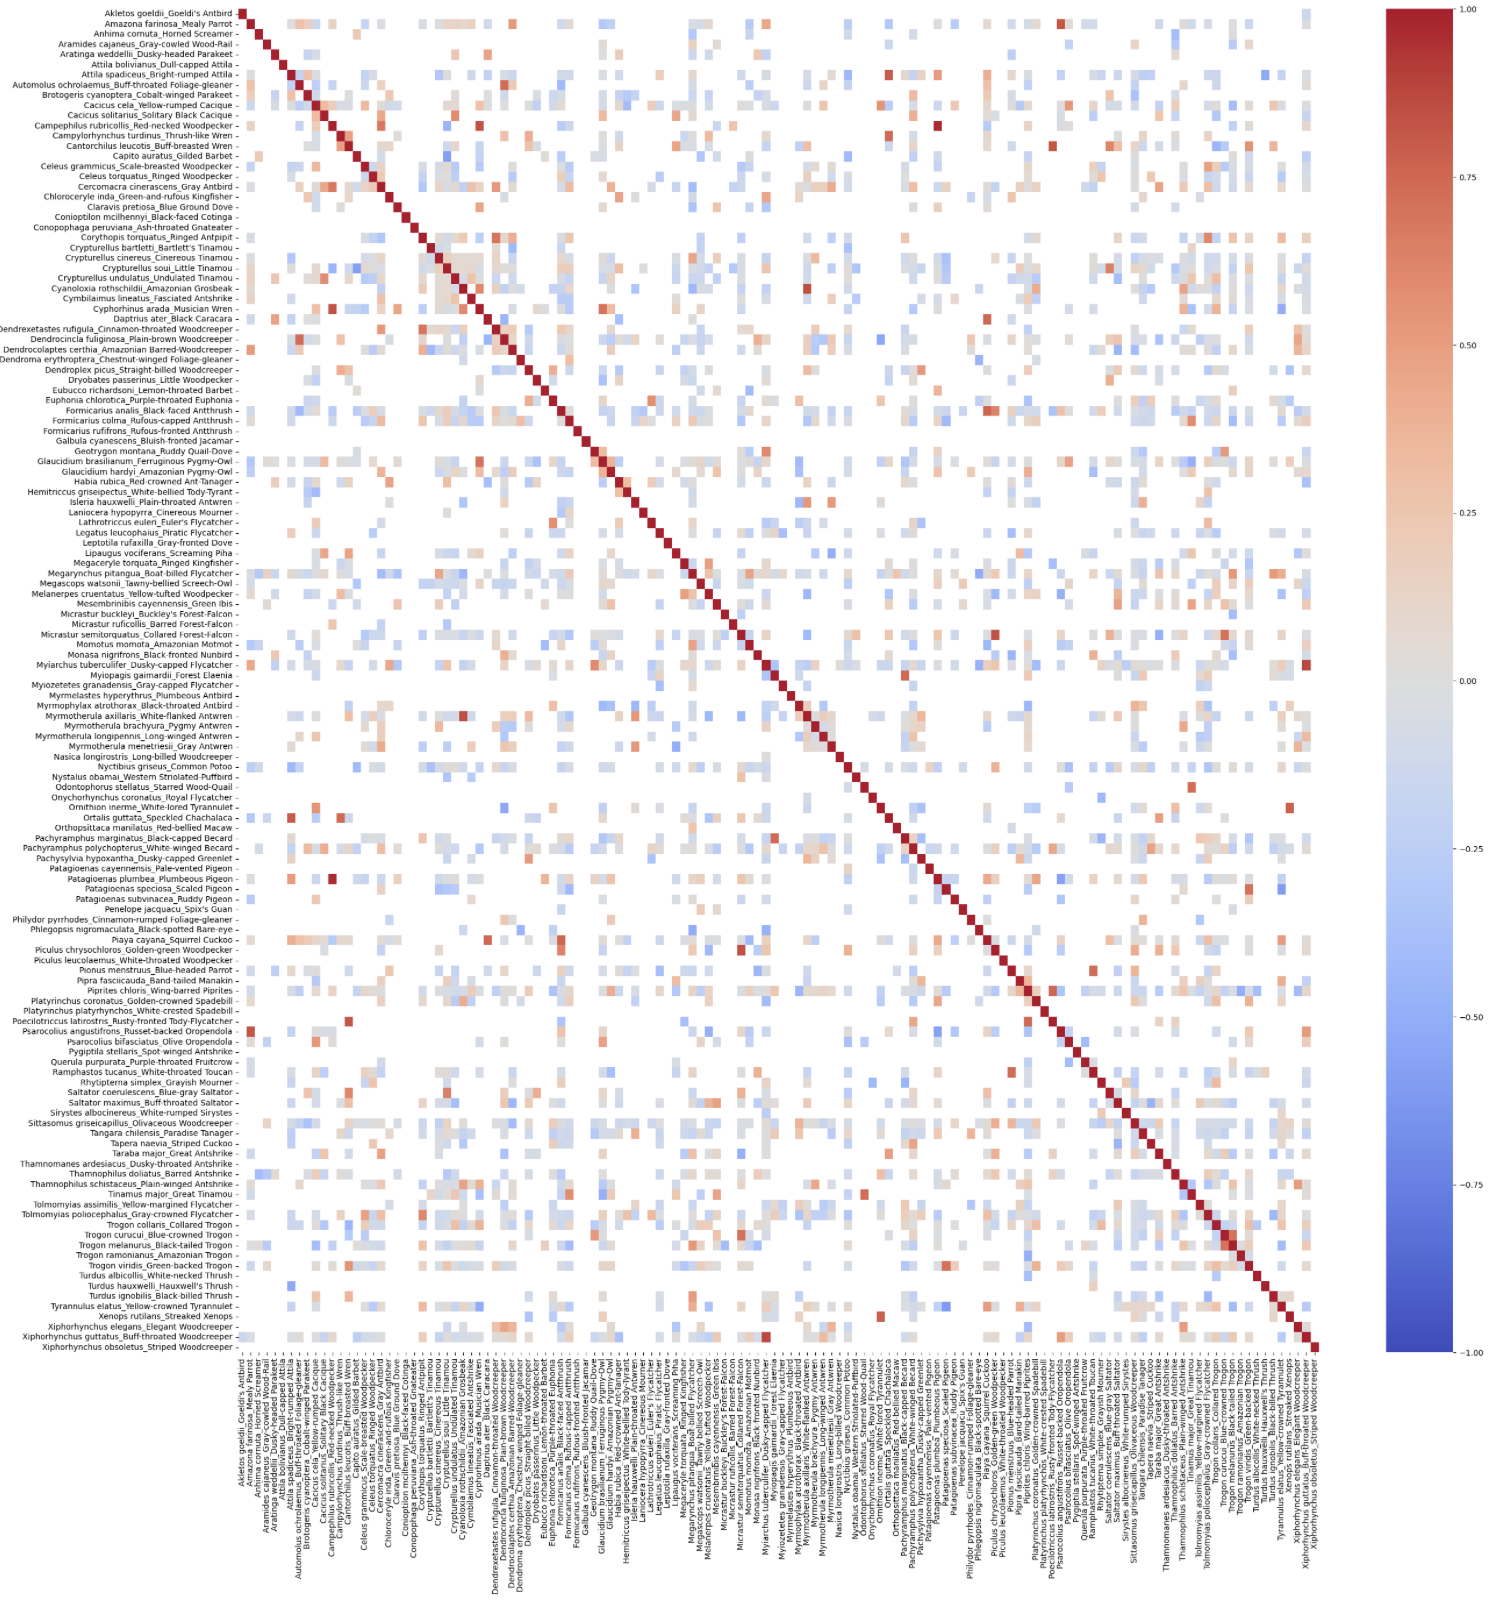
\includegraphics[height=0.9\textheight,width=0.9\textwidth,keepaspectratio]{images/occurance_filter.png}   
\end{frame}

% picture of matrix, with filtering the number of datapoints
\begin{frame}{Results: Class Correlation Matrix}
    \centering
    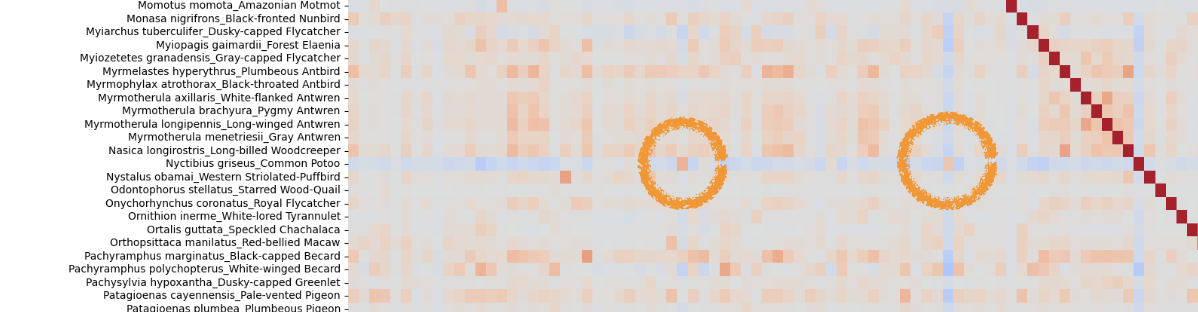
\includegraphics[height=0.9\textheight,width=0.9\textwidth,keepaspectratio]{images/night.png}   
\end{frame}

% Initial analysis: night vs. day & similar species
% To create a slide with two columns, use the following:
\begin{frame}{TITLE}
    \begin{columns}
        \begin{column}{0.5\textwidth}
            \centering
            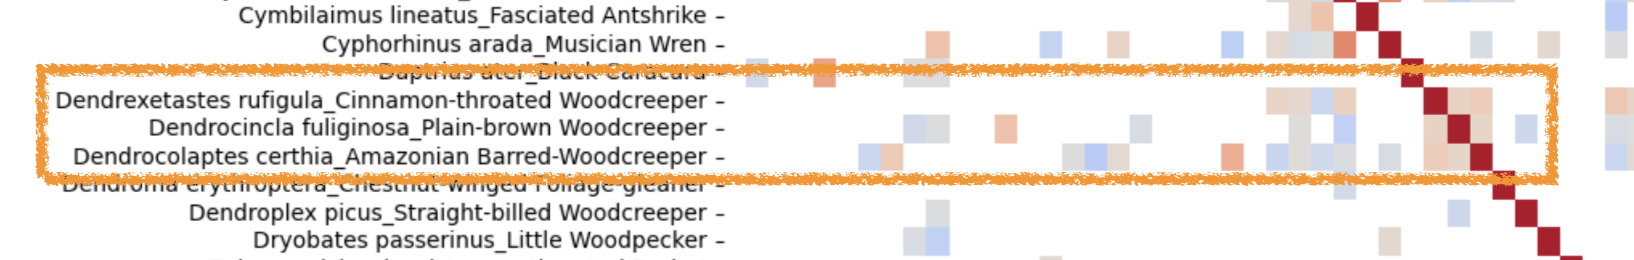
\includegraphics[height=0.9\textheight,width=0.9\textwidth,keepaspectratio]{images/sim1.png}   
        \end{column}
        \begin{column}{0.5\textwidth}
            \centering
            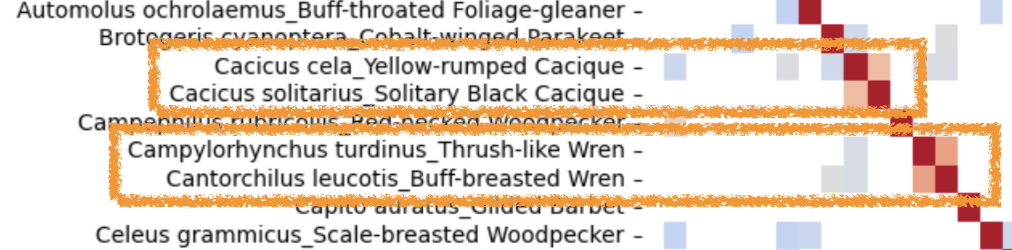
\includegraphics[height=0.9\textheight,width=0.9\textwidth,keepaspectratio]{images/sim2.png} 
        \end{column}
    \end{columns}
\end{frame}

% Begin TQ's section
\begin{frame}{Correlation Graph}
    \centering Idea: Use correlations as adjacency
\end{frame}

\begin{frame}{Interactive Graph Visualization}
    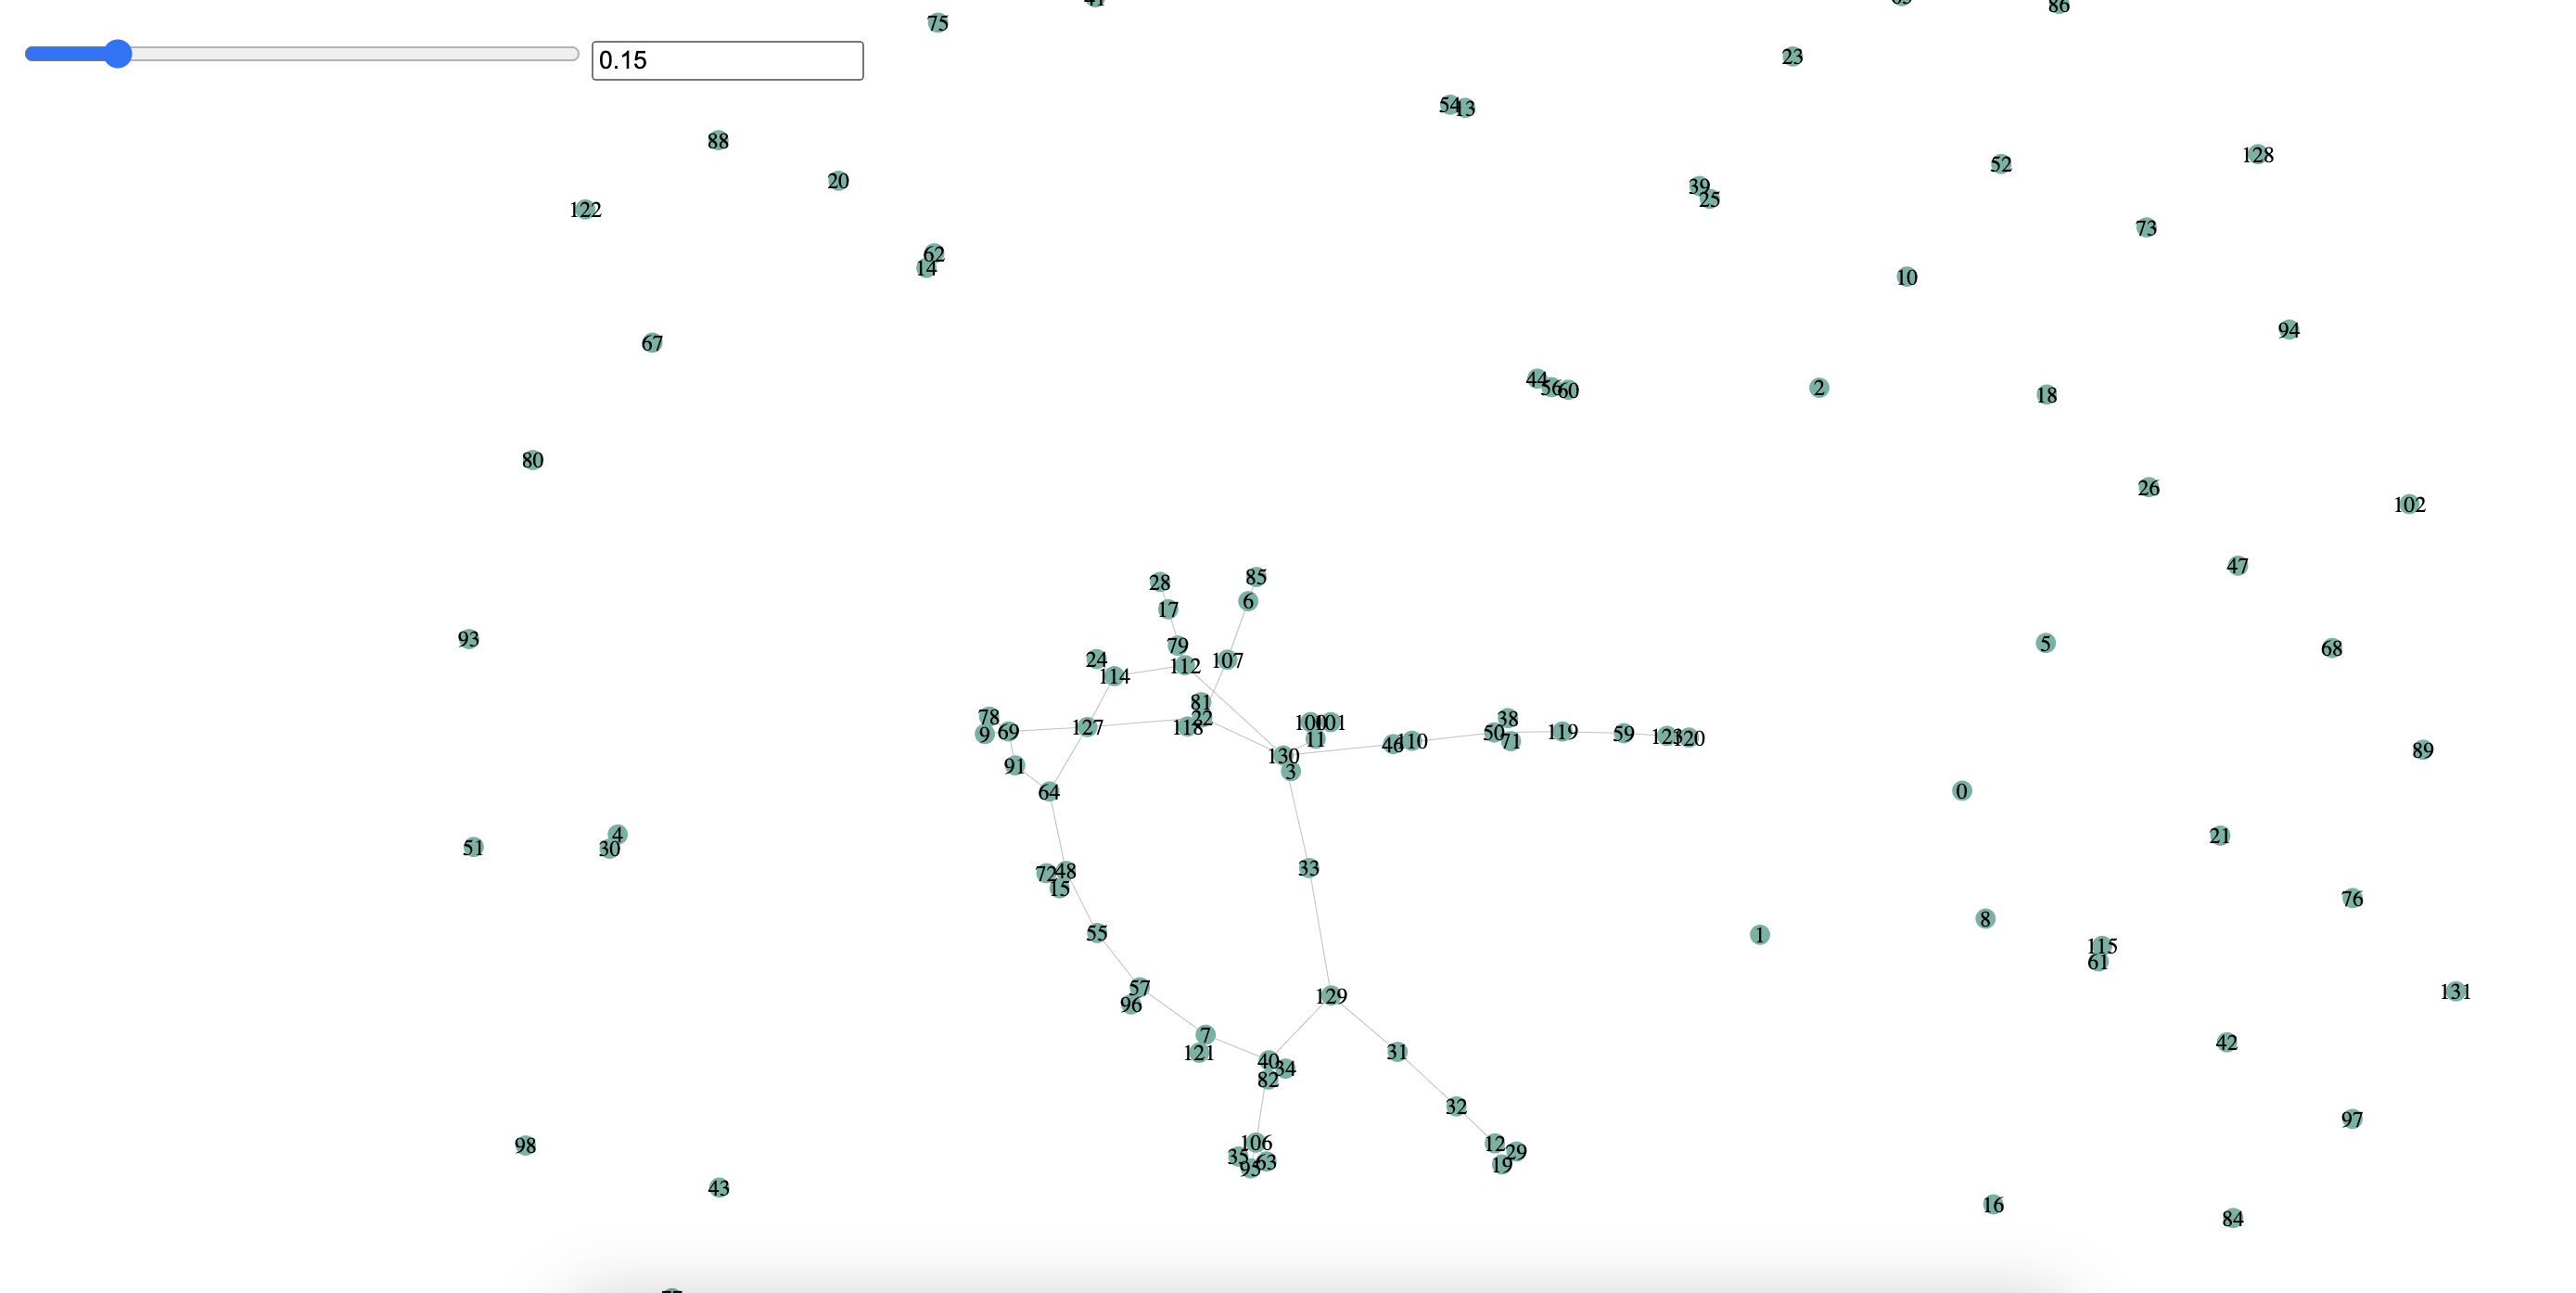
\includegraphics[height=0.9\textheight, width=0.9\textwidth]{images/asid_corr_graphvis.png}
\end{frame}

\begin{frame}{Groups Make Sense}
    \begin{columns}
        \begin{column}{0.5\textwidth}
            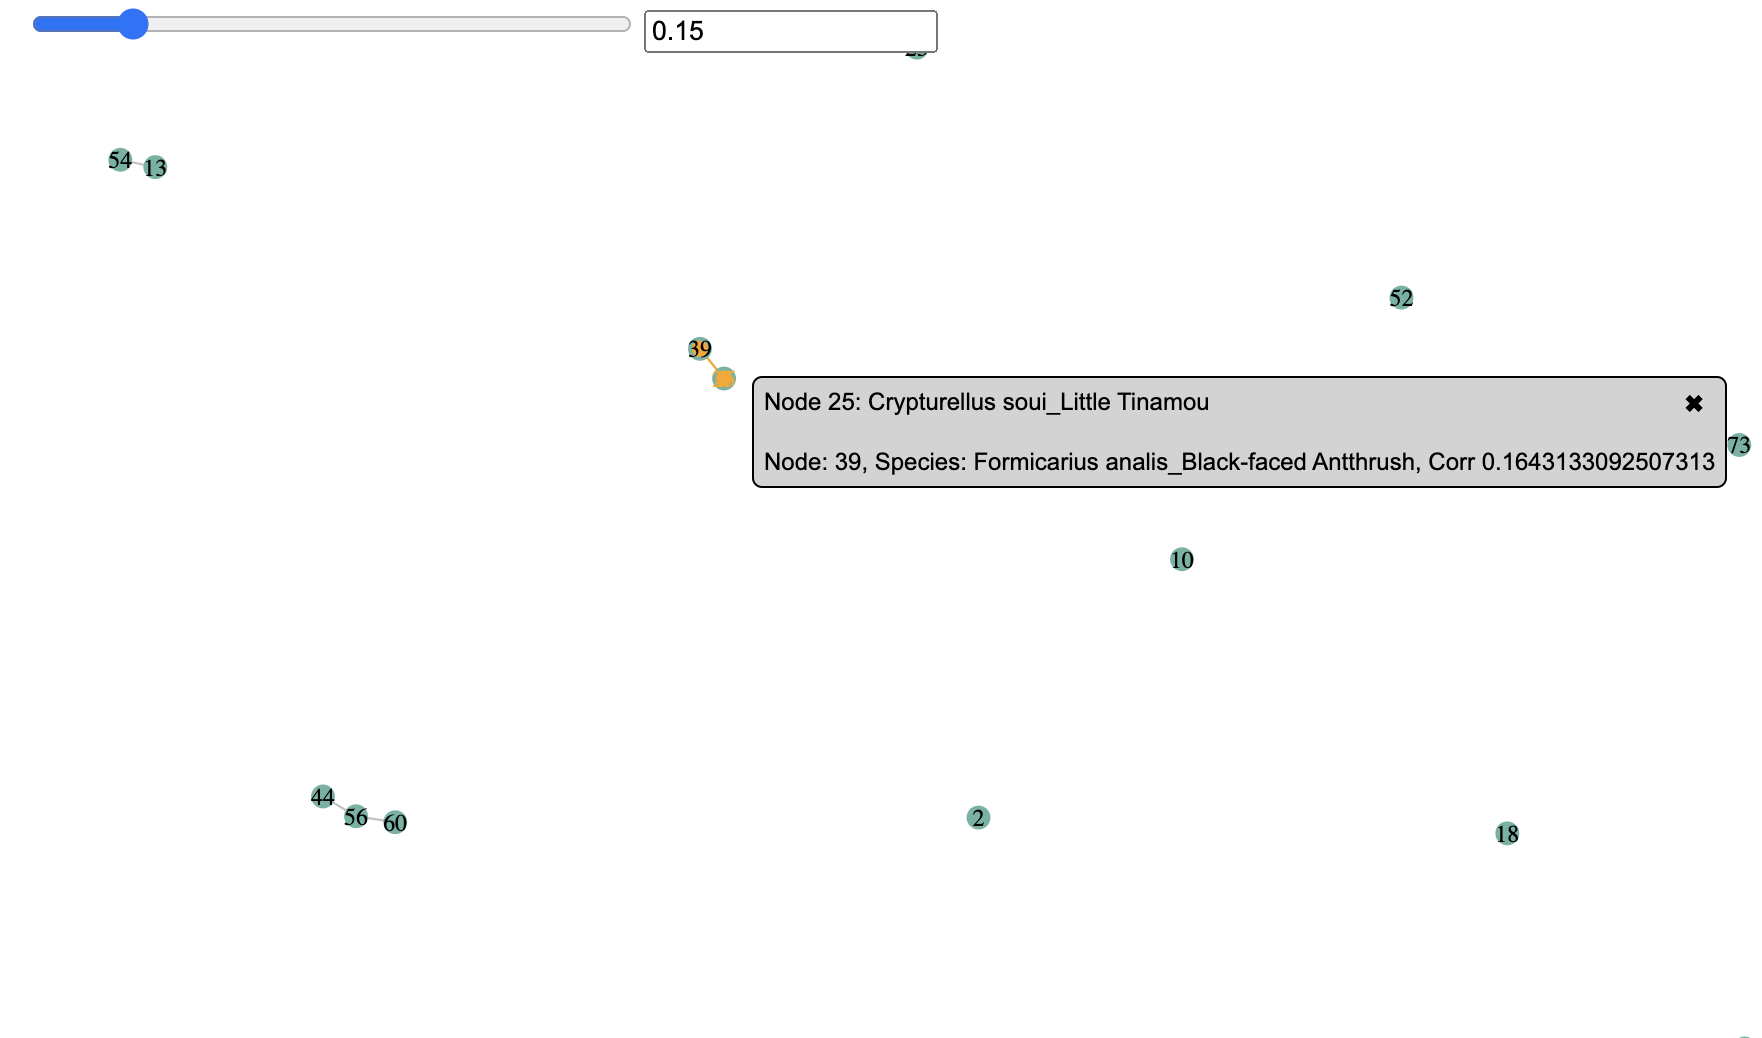
\includegraphics[height=0.7\textheight, width=1\textwidth]{images/antthrush_tinamou.png}
        \end{column}
        \begin{column}{0.5\textwidth}
            \begin{itemize}
                \item Black-faced Antthrush: https://xeno-canto.org/712297
                \item Little Tinamou: https://xeno-canto.org/821655
            \end{itemize}
        \end{column}
    \end{columns}
\end{frame}

\begin{frame}{Interpretation/Future application}
    \begin{itemize}
        \item Model confusion makes sense
        \item See where it's getting confused
    \end{itemize}
\end{frame}

% To create a slide with numbered list, use the following:
% \begin{frame}{TITLE}
%     \begin{enumerate}
%         \item ITEM 1
%         \item ITEM 2
%     \end{enumerate}
% \end{frame}

% To create a slide with a graphic:
% 1. Add the graphic to this folder (named picture.png)
% 2. Use the following:
% \begin{frame}{TITLE}
%     \centering
%     \includegraphics[height=0.7\textheight,width=0.7\textwidth,keepaspectratio]{picture.png}
% \end{frame}

% To create a slide with two columns, use the following:
% \begin{frame}{TITLE}
%     \begin{columns}
%         \begin{column}{0.5\textwidth}
%             COLUMN 1 BODY
%         \end{column}
%         \begin{column}{0.5\textwidth}
%             COLUMN 2 BODY
%         \end{column}
%     \end{columns}
% \end{frame}

%surangana's part

\begin{frame}{Past week}  
    \begin{itemize}
        \item Data Analysis
    \end{itemize}
    \centering
    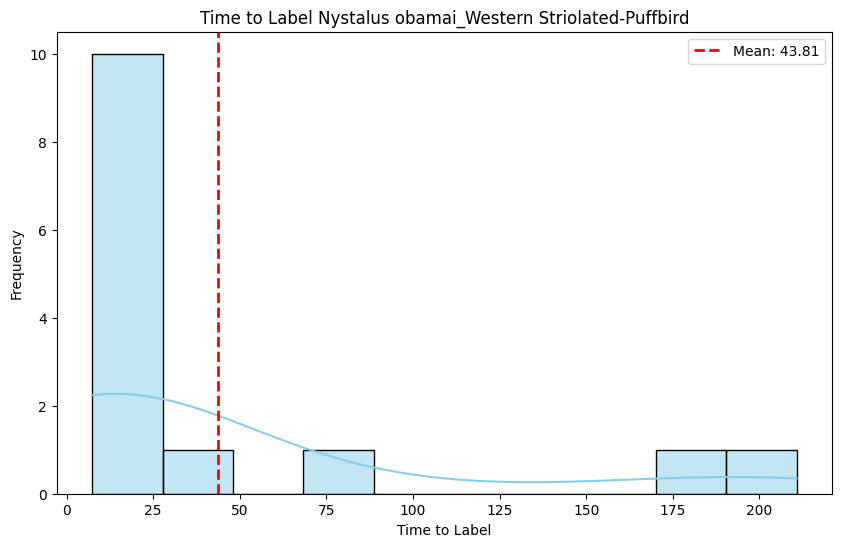
\includegraphics[width=0.6\textwidth]{images/data analysis.png}  
\end{frame}

\begin{frame}{Past week} 
    \begin{itemize}
        \item Created Sample UI Designs
    \end{itemize}  
    \centering
    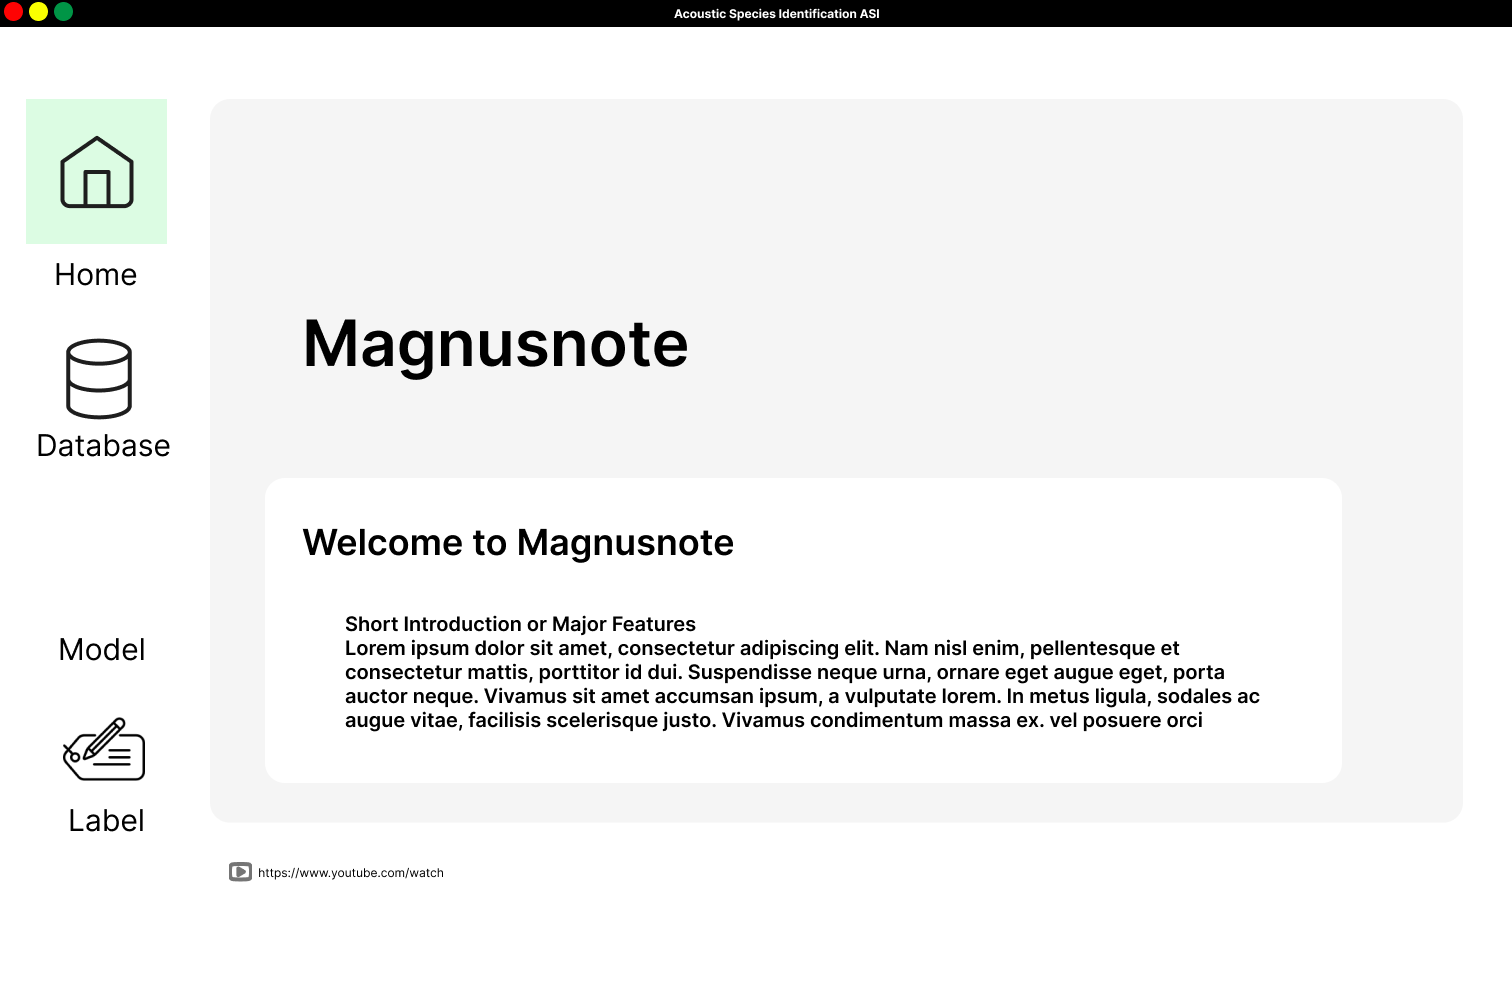
\includegraphics[width=0.6\textwidth]{images/sampleui1.png}  
\end{frame}

\begin{frame}{Past week} 
    \begin{minipage}[b]{0.45\textwidth}
        \centering
        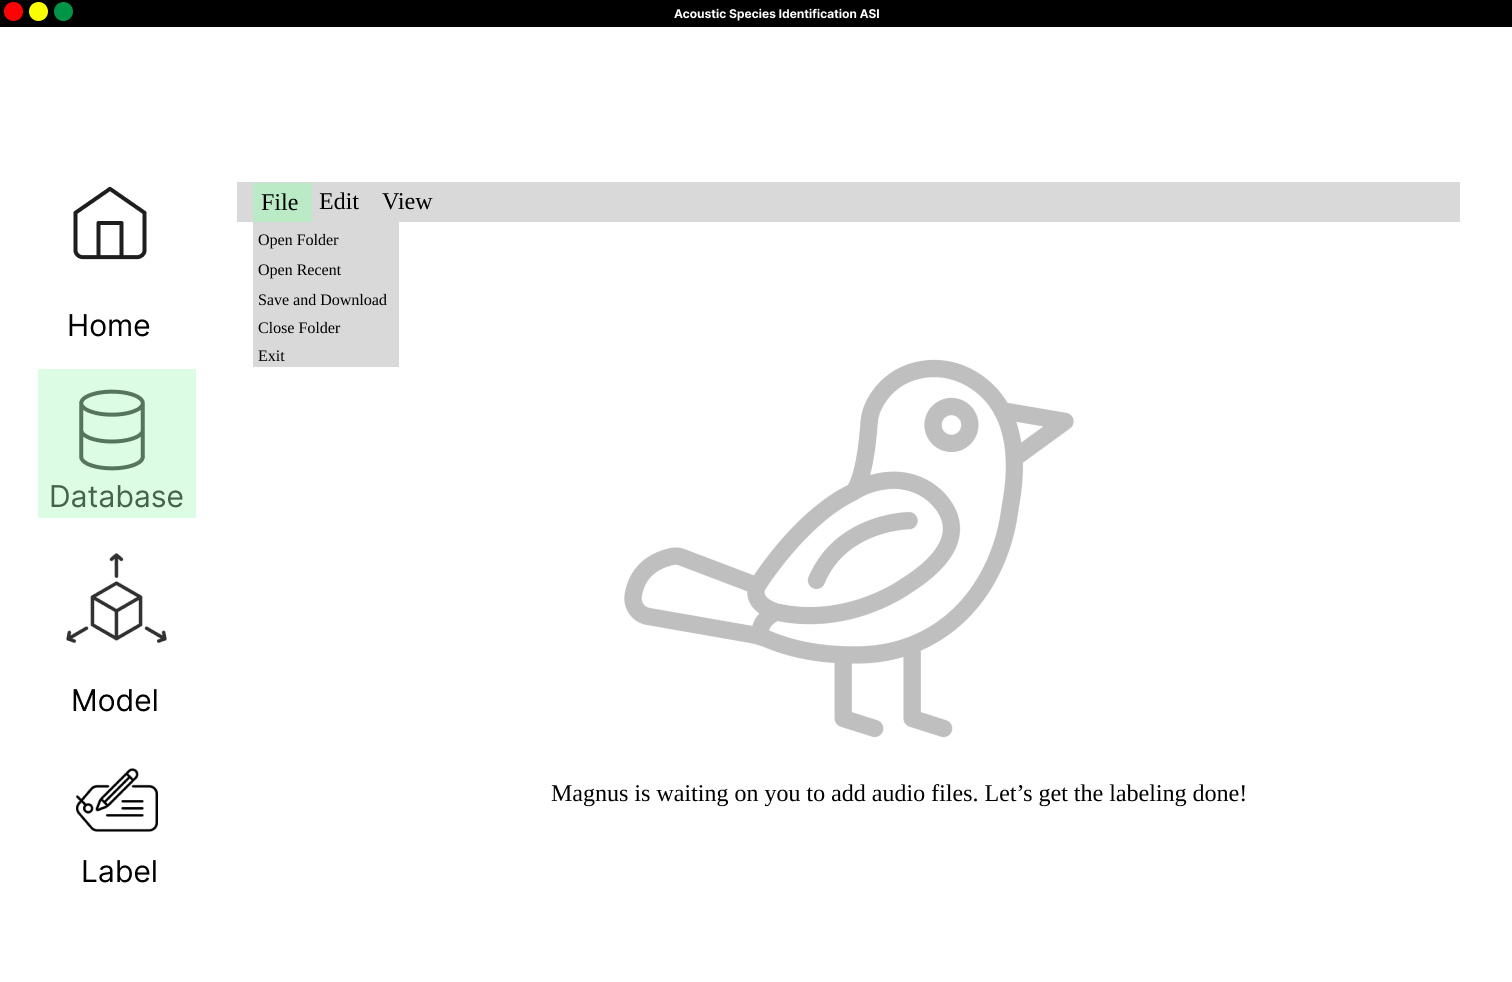
\includegraphics[width=\textwidth]{images/sampleui2.png}  
    \end{minipage}
    \hspace{0.05\textwidth}
    \begin{minipage}[b]{0.45\textwidth}
        \centering
        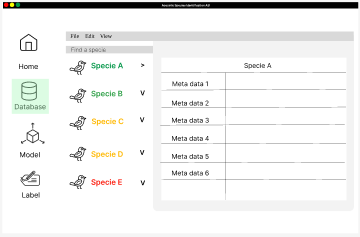
\includegraphics[width=\textwidth]{images/sampleui5.png} 
    \end{minipage}
\end{frame}

\begin{frame}{Past week} 
    \begin{minipage}[b]{0.45\textwidth}
        \centering
        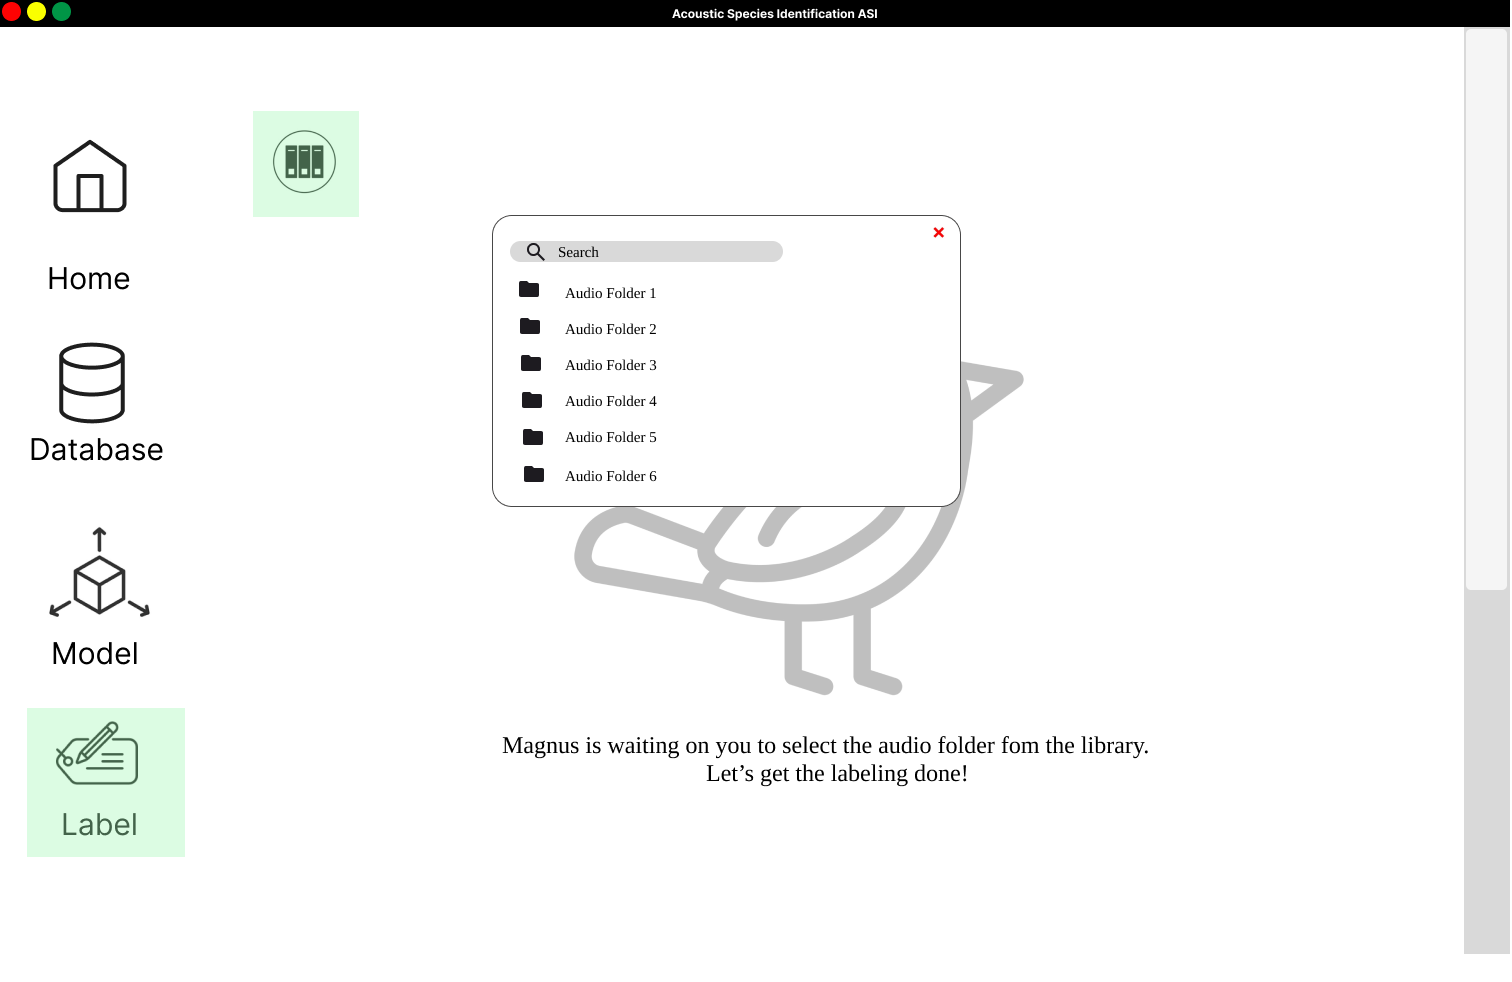
\includegraphics[width=\textwidth]{images/sampleui4.png}  
    \end{minipage}%
    \hspace{0.05\textwidth}
    \begin{minipage}[b]{0.45\textwidth}
        \centering
        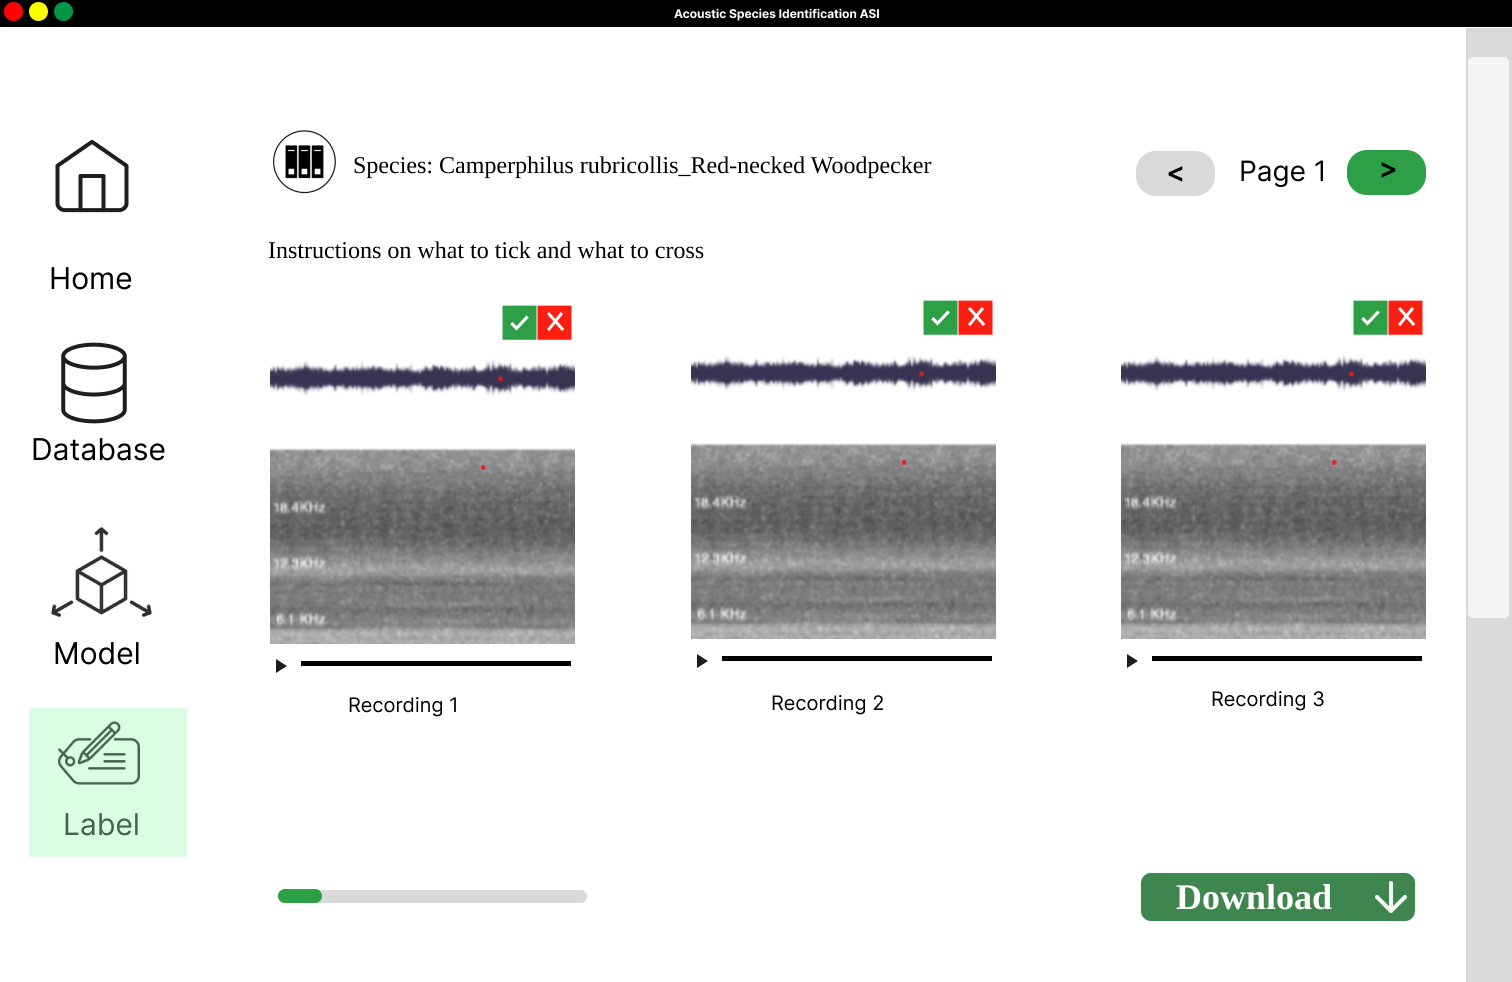
\includegraphics[width=\textwidth]{images/sampleui3.png}  
    \end{minipage}
\end{frame}

\begin{frame}{Upcoming week} 
    \begin{itemize}
        \item Iterate the designs 
    \end{itemize}  
\end{frame}